\documentclass[a4paper,12pt]{article} %style de document
\usepackage[utf8]{inputenc} %encodage des caractères
\usepackage[french]{babel} %paquet de langue français
\usepackage[T1]{fontenc} %encodage de la police
\usepackage[top=2cm,bottom=2cm,left=2cm,right=2cm]{geometry} %marges
\usepackage{graphicx} %affichage des images
\usepackage{amssymb}
\usepackage{url}
\usepackage{verbatim}
\usepackage{amsmath}

\begin{document} %début du document



%----------------------------------
%page de garde
%----------------------------------

\begin{titlepage}

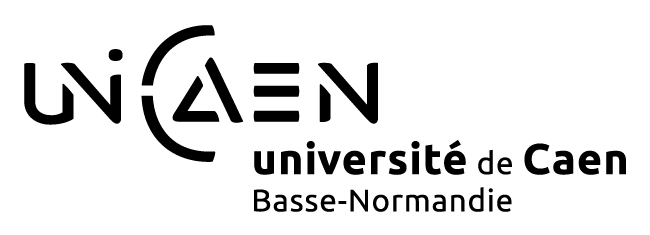
\includegraphics[scale=0.3]{images/unicaen.png}

\vspace{7cm}

\begin{center}

\begin{Huge}
Sécurité et Aide à la Décision\\
Expérimentations du TP\\
\end{Huge}
\vspace{2cm}
\begin{large}
Mori Baptiste 21602052\\
Leblond Valentin 21609038\\
\vspace{1cm}
L2-Info-groupe-4A
\end{large}

\end{center}
\end{titlepage}


%------------------------------
%sommaire
%------------------------------

\newpage

\tableofcontents{}

\newpage

%------------------------------
%contenu
%------------------------------


\section*{Introduction}
\addcontentsline{toc}{section}{Introduction}

L'objectif de ce TP est de mettre en place deux intelligence artificielles, la première fonctionnant avec l'algorithme Minmax et l'autre avec l'algorithme Alphabeta. Ces intelligences artificielles nous servirons à choisir le meilleurs coup à jouer sur une profondeur donnée.

Nous allons procéder à des expérimentation sur le nombre de nœuds que parcours chaque algorithme afin de comparer Minmax et Alphabeta.

\section{Tests sur le nombre de parcours des nœuds}

Nous allons nous intéresser à comparer le nombre de nœuds que parcourt chaque algorithme. Pour cela, nous avons implémenté un compteur dans le constructeur de la classe de L'IA afin de compter chaque passage dans Minmax et dans Alphabeta.\\

Dans un premier temps, nous allons faire varier le nombre de profondeur auquel les algorithme vont regarder tout en gardant le même graph de départ pour le test de chaque profondeur. Nous utiliseront Matplotlib et Numpy pour construire nos graphiques.

\begin{center}
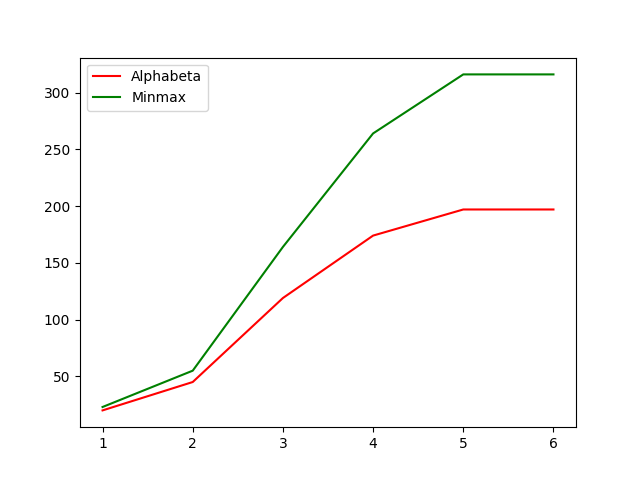
\includegraphics[scale=0.5]{images/Figure_1.png}
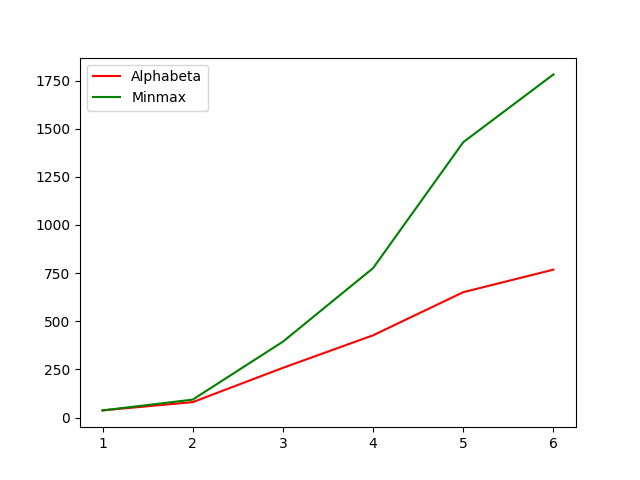
\includegraphics[scale=0.5]{images/Figure_2.png}
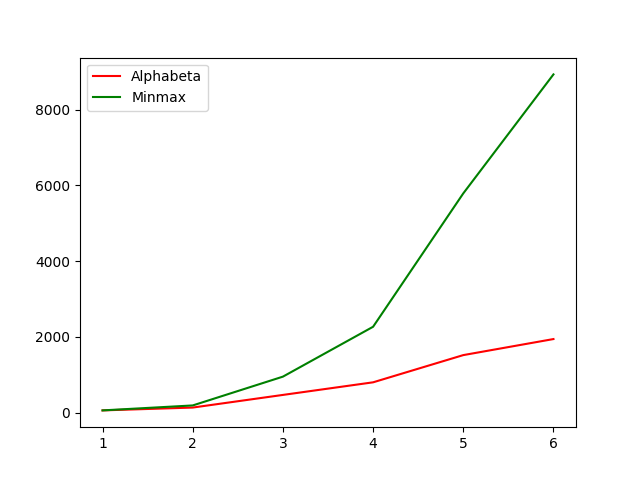
\includegraphics[scale=0.5]{images/Figure_3.png}\\
Nombre de nœuds parcourus en fonction de la profondeur
\end{center}

On remarque que pour chaque test, Alphabeta est toujours bien en dessous en terme de parcours que Minmax, même si pour le premier graphique le graph du jeu semble un peux particulier (le passage entre la profondeur 5 et 6 n'a pas changer énormément le nombre de parcours), Alphabeta semble parcourir le moins de nœuds quelque soit la profondeur qu'on lui donne.\\

Dans un second temps, nous allons faire varier la probabilité que deux ordinateurs soient connectés (cette fois nous recréons à chaque fois un nouveau graph d'où les courbes un peu chaotique).

\begin{center}
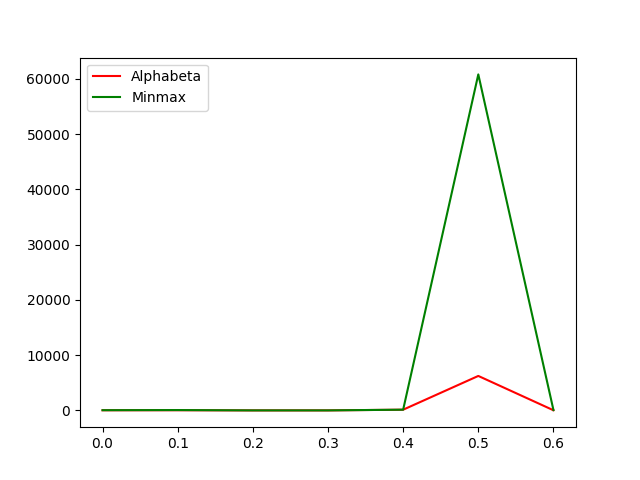
\includegraphics[scale=0.5]{images/Figure_4.png}
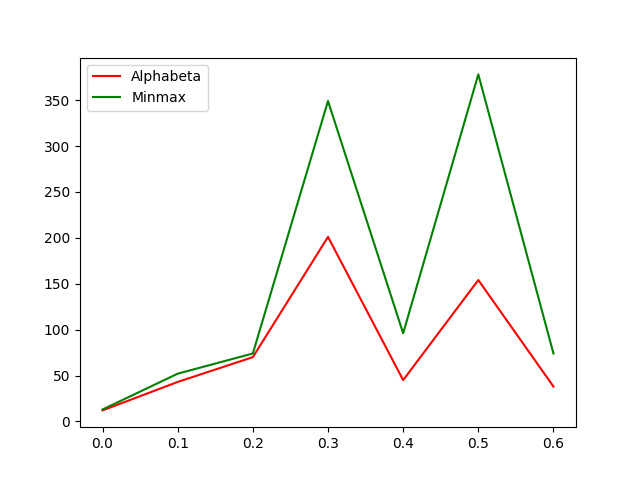
\includegraphics[scale=0.5]{images/Figure_5.png}
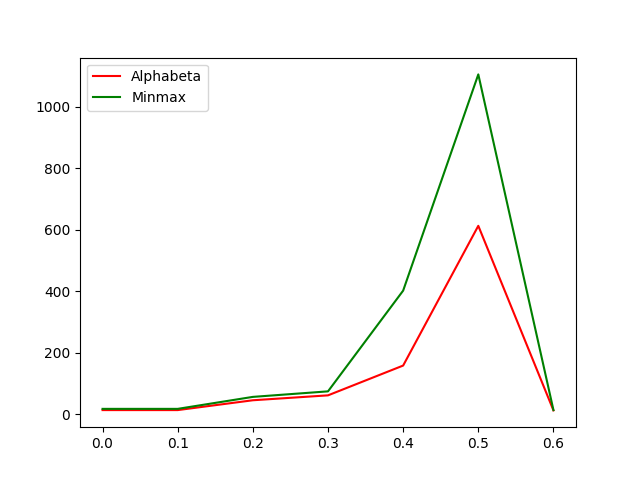
\includegraphics[scale=0.5]{images/Figure_6.png}\\
Nombre de nœuds parcourus en fonction de la probabilité
\end{center}

On remarque de même que Alphabeta parcours moins de nœuds que Minmax et que plus Minmax parcours de nœuds, plus l'écart entre les deux est important, il y a donc une relation de puissance sur le nombre de nœuds parcourus par ces deux algorithmes. On remarque également quand Minmax parcours très peu de nœuds (<50 nœuds environ), il arrive que Minmax et Alphabeta parcours le même nombre de nœuds comme on peut le voir sur la capture suivante avec Alphabeta en haut et Minmax en dessous.

\begin{center}
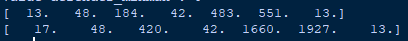
\includegraphics[scale=1]{images/Capture.PNG}
\end{center}

\section*{Conclusion}
\addcontentsline{toc}{section}{Conclusion}

Minmax et Alphabeta prenant la même décision du meilleur coup, Alphabeta est celui qui parcours le moins de nœuds et donc qui est le plus rapide dans sa prise de décision que se soit par l'augmentation de la profondeur de raisonnement mais aussi par l'augmentation du nombre de possibilités de coup à jouer, dans notre cas la probabilité que deux ordinateurs soient connectés.

\end{document}
